% Undergraduate dissertation, Wenzhou-Kean University.
\documentclass[11pt,a4paper,oneside]{report}
\usepackage[T1]{fontenc}
\usepackage[utf8]{inputenc}
\usepackage{lmodern}
\usepackage[nopatch=footnote]{microtype}
\usepackage[margin=27mm,headheight=14pt]{geometry}
\usepackage{amsmath,amssymb,amsthm,mathtools}
\usepackage{booktabs,longtable,array,tabularx}
\renewcommand{\tabularxcolumn}[1]{>{\raggedright\arraybackslash}p{#1}}
\usepackage{graphicx,tikz,pgfplots,float}
\usetikzlibrary{arrows.meta,positioning,calc,fit,backgrounds,decorations.markings}
\pgfplotsset{compat=1.18}
\usepackage[numbers,sort&compress]{natbib}
\usepackage[hyphens]{url}
\usepackage{hyperref,bookmark}
\usepackage{listings,setspace,fancyhdr,titlesec,caption}
\titleformat{\chapter}[hang]{\normalfont\Large\bfseries}{\thechapter}{1em}{}
\titlespacing*{\chapter}{0pt}{0pt}{16pt}
\titleformat{\section}{\normalfont\large\bfseries}{\thesection}{.7em}{}
\titlespacing*{\section}{0pt}{12pt plus 2pt}{5pt}
\captionsetup{font=small,labelfont=bf,skip=5pt}
\setlength{\textfloatsep}{12pt plus 2pt minus 2pt}
\setlength{\intextsep}{10pt plus 2pt minus 2pt}
\renewcommand{\topfraction}{.9}
\renewcommand{\bottomfraction}{.8}
\renewcommand{\textfraction}{.08}
\definecolor{ink}{HTML}{24345C}
\definecolor{teal}{HTML}{147D86}
\definecolor{warm}{HTML}{B76032}
\hypersetup{hidelinks,pdftitle={Verified Lie Reductions and Symmetry-Guided Constitutive Models for SVE-Type Equations}}
\setstretch{1.08}
\setlength{\emergencystretch}{3em}
\setlength{\parskip}{2pt}\raggedbottom
\setcounter{tocdepth}{1}
\numberwithin{equation}{chapter}
\newtheorem{theorem}{Theorem}[chapter]
\newtheorem{proposition}[theorem]{Proposition}
\newtheorem{definition}[theorem]{Definition}
\newtheorem{remark}[theorem]{Remark}
\newcommand{\E}{\mathcal E}
\newcommand{\R}{\mathcal R}
\newcommand{\dd}{\mathrm d}
\newcommand{\pr}{\operatorname{pr}}
\newcommand{\rank}{\operatorname{rank}}
\newcommand{\norm}[1]{\left\lVert#1\right\rVert}
\DeclareRobustCommand{\code}[1]{\nolinkurl{#1}}
\lstset{basicstyle=\footnotesize\ttfamily,breaklines=true,columns=fullflexible,frame=single,keepspaces=true,showstringspaces=false}
\tikzset{box/.style={draw=ink,fill=ink!4,rounded corners=3pt,align=center,inner sep=5pt,font=\small},arr/.style={-{Latex[length=2.4mm]},thick,ink},note/.style={font=\small,align=center},every picture/.style={line cap=round}}
\pagestyle{fancy}\fancyhf{}\fancyhead[L]{\small\nouppercase{\leftmark}}\fancyfoot[C]{\thepage}
\renewcommand{\chaptermark}[1]{\markboth{\thechapter.\ #1}{}}
\begin{document}
\begin{titlepage}
\centering
{\large Wenzhou--Kean University\par}
\vspace{12mm}
{\large Undergraduate Dissertation\par}
\vspace{25mm}
{\LARGE\bfseries Verified Lie Symmetry Reductions\par}
\vspace{4mm}
{\LARGE\bfseries and Symmetry-Guided Constitutive Modelling\par}
\vspace{10mm}
{\Large Saint--Venant--Exner-Type Equations\par}
\vspace{15mm}
{\large Geometric foundations and semi-analytical computation\par}
\vfill
{\large 27 October 2026\par}
\end{titlepage}
\pagenumbering{roman}
\graphicspath{{draft/figures/final-20261027/}{figures/final-20261027/}}
\chapter*{Abstract}\addcontentsline{toc}{chapter}{Abstract}
Lie symmetry is useful when reduction preserves the equation, parameter conditions and physical interpretation. This dissertation audits a scalar Saint--Venant--Exner benchmark and distinguishes the printed scalar equation, a corrected material equation and the full Eulerian flow--bed system. A worked scaling reduction derives invariants, a reduced equation, a first integral and local reconstruction. Exact witnesses identify errors in displayed source formulas.

An equation-first symbolic pipeline independently checks returned generator families and selected pullback identities. Thirty declared inputs were attempted. After the generic one-dimensional Grass input timed out, a direct determining-equation formulation returned a verified four-dimensional algebra on a restricted parameter chart. Its exceptional layers remain unresolved, as does exhaustive classification. A separate annular two-dimensional reference has exact reduction and sampled numerical verification. In a mixed sediment law, joint rotation survives while the old cubic scaling fails. These results support local analytical claims and reproducible negative findings, without universal reduction, experimental calibration or neural-superiority claims.
\tableofcontents\clearpage\pagenumbering{arabic}
\chapter{Introduction}\label{ch:intro}
\section{Physical problem and mathematical question}
A moving water layer transports sediment and changes the bed over which it flows. The changed bed modifies the pressure gradient and therefore the subsequent flow. Saint--Venant--Exner (SVE) models express this feedback through coupled water and sediment balances. Their usefulness depends on the depth-averaging assumptions, constitutive law, boundary data, and temporal and spatial scales. An exact solution of a simplified equation is valuable as an analytical reference, but its existence alone does not validate that equation for a particular sediment experiment.

This dissertation asks when symmetry analysis supplies a valid reduction, when that reduction improves computation, and whether the same determining equations can constrain an unknown sediment law. The classical geometric foundation follows Olver \cite{olver,olver1986} and Oliveri \cite{oliveri2026}. The direct scalar benchmark is the Lagrangian shallow-water equation studied by Paliathanasis, Leon, and Leach \cite{ap}. The more recent enforce--discover--promote framework of Otto et al.\ \cite{otto} motivates a separate extension toward model identification.

\section{Research questions and contributions}
The argument is organized around four questions. First, which scalar representation can be reconstructed into the stated Eulerian equations? Second, which group actions admit regular invariant graphs and compatible data? Third, after an exact first integral has removed one derivative order, what numerical task remains? Fourth, what information about an unknown constitutive function can be obtained from a prescribed symmetry?

Chapter 2 reproduces the model transformations and a complete selected reduction. Chapter 3 explains discrepancies, acceptance gates and algorithmic improvements. Chapter 4 tests two-dimensional and constitutive extensions. Chapter 5 states supported conclusions and the next falsifiable tasks. The results concern smooth local branches, not shock theory, maximal multidimensional classification or physically calibrated learned laws.

\begin{equation*}
\text{Model}\;\longrightarrow\;\text{Symmetry}\;\longrightarrow\;\text{Reduction}
\;\longrightarrow\;\text{Reconstruction and validation}.
\end{equation*}
Observation-based validation can motivate a revised closure; it does not follow from equation symmetry alone.


\section{Scope of the literature and of the evidence}
Classical Lie theory describes transformations of equations and their invariant solutions \cite{olver,oliveri2026}. Nontransverse actions need additional treatment \cite{anderson2000}. Neural solution representations may impose initial data analytically \cite{lagaris}; symmetry-informed neural losses \cite{sympinn} and approximation error analysis \cite{mishra2023} address related but distinct issues. None of these sources establishes that a neural method must outperform a classical solver after reduction to a regular one-dimensional ODE.

\chapter{Reproduction}\label{ch:models}\label{ch:reduction}
\section{Conservation equations and constitutive assumptions}
For smooth fields on an open spacetime region, take $h(t,x)>0$, velocity $u(t,x)$, bed elevation $B(t,x)$, and fixed $g>0$. The effective flux $q$ absorbs a constant sediment porosity factor. The one-dimensional frictionless model without external forcing is
\begin{align}
h_t+(hu)_x&=0,\label{eq:e1}\\
(hu)_t+(hu^2+\tfrac12gh^2)_x+ghB_x&=0,\label{eq:e2}\\
B_t+\partial_xq(h,u)&=0.\label{eq:e3}
\end{align}
The second equation is a momentum balance with a bed-slope source; its nonconservative product requires additional specification across discontinuities. Here all calculations are classical. On $h>0$, subtracting $u$ times \eqref{eq:e1} from \eqref{eq:e2} gives $u_t+uu_x+g(h+B)_x=0$.

For the power-law benchmark, $q=\kappa u^m$ on $u>0$, with $\kappa>0$, $m\ge1$ and $\beta=m\kappa$. Fractional real exponents are smooth on this positive branch. Reversed flow requires a separately specified signed law; it is not covered by silently extending $u^m$ to negative $u$.

\begin{figure}[htbp]\centering
\begin{tikzpicture}[x=1cm,y=1cm]
\fill[teal!12] (0,.7) .. controls (3,.1) and (6,1.3) .. (10,.65) -- (10,2.8) -- (0,2.8)--cycle;
\fill[warm!20] (0,-.1)--(10,-.1)--(10,.65)..controls(6,1.3)and(3,.1)..(0,.7)--cycle;
\draw[very thick,warm] (0,.7)..controls(3,.1)and(6,1.3)..(10,.65);
\draw[thick,teal] (0,2.8)--(10,2.8);
\draw[arr] (2,1.8)--(4.2,1.8) node[midway,above]{$u(t,x)$};
\draw[arr,warm] (5,.45)--(7,.65) node[midway,below=3pt]{$q(h,u)$};
\draw[<->,thick] (8,.85)--(8,2.8) node[midway,right]{$h$};
\draw[dashed] (0,-.1)--(10,-.1);
\draw[<->] (.6,-.1)--(.6,.6) node[midway,left]{$B$};
\node[note,above] at (5,2.8){free surface $h+B$};
\draw[arr] (0,-.65)--(10,-.65) node[right]{$x$};
\end{tikzpicture}
\caption{Depth-averaged flow and sediment transport (schematic).}\label{fig:physical}
\end{figure}

\paragraph{Second-order extension.}
A possible downslope closure replaces \eqref{eq:e3} by
\begin{equation}\label{eq:diffusive}
B_t+\partial_x\{q(h,u)-G_0u^nB_x\}=0,\qquad G_0>0,\quad u>0.
\end{equation}
Its highest bed derivative is $-G_0u^nB_{xx}$, a positive diffusion coefficient in evolution form. This extension is absent from this chapter's scalar $P$ experiments. Under the fixed-parameter scaling \eqref{eq:euler-scale}, the diffusive flux has weight $n+1$, whereas the required flux weight is $3$; hence this particular scaling requires $n=2$. A different generator or a transformation of $G_0$ defines a different symmetry question.

\section{Material coordinates and the E/M/P distinction}
Continuity implies that $h\,\dd x-hu\,\dd t$ is locally exact. Thus a mass label satisfies $s_x=h$ and $s_t=-hu$. Inverting $s(t,x)$ locally gives $x=\phi(t,s)$, with
\begin{equation}
\phi_s=1/h(t,\phi)>0,\qquad \phi_t=u(t,\phi).
\end{equation}
For $f^L(t,s)=f(t,\phi(t,s))$,
\begin{equation}\label{eq:chain}
\partial_x=\phi_s^{-1}D_s,\qquad
\partial_t\big|_x=D_t\big|_s-\frac{\phi_t}{\phi_s}D_s.
\end{equation}
These are operator identities on pulled-back fields. The label $s$ has units of area per unit transverse width when $s_x=h$; it is not an ordinary spatial distance. The formulas may also be read in consistent nondimensional variables.

Writing $b(t,s)=B(t,\phi(t,s))$, define
\begin{equation}
A=\phi_s\phi_{tt}-g\frac{\phi_{ss}}{\phi_s^2},\qquad
T_m=\frac{\phi_t^{m-1}\phi_{ts}}{\phi_s}.
\end{equation}
The pulled-back momentum and bed equations are
\begin{equation}\label{eq:coupled}
A+gb_s=0,\qquad b_t-\frac{\phi_t}{\phi_s}b_s+\beta T_m=0.
\end{equation}
The coupled system \eqref{eq:coupled} is second order in $\phi$ and first order in $b$. For \eqref{eq:diffusive}, the bed equation instead contains
\begin{equation}\label{eq:diffusive-material}
b_t-\frac{\phi_t}{\phi_s}b_s+\beta T_m
-\frac{G_0}{\phi_s}D_s\!\left(\frac{\phi_t^n b_s}{\phi_s}\right)=0.
\end{equation}
Thus second-order coupled models are already present before scalar elimination. The scalar equations below concern $G_0=0$ only.
Compare the printed scalar equation with the compatibility equation obtained by equating the mixed derivatives of $b$:
\begin{align}
\E_m^{\mathrm p}&=D_tA-g\beta D_sT_m=0 &&\text{(model $P$)},\label{eq:printed}\\
\E_m^{\mathrm c}&=D_tA-g\beta D_sT_m-D_s\!\left(\frac{\phi_t}{\phi_s}A\right)=0 &&\text{(model $M$)}.\label{eq:corrected}
\end{align}
Model $P$ is the printed scalar benchmark of Paliathanasis, Leon and Leach \cite{ap}; model $M$ is the compatibility equation obtained from \eqref{eq:coupled}. They coincide only on additional restricted fields for which the extra divergence vanishes. A coordinate change alone cannot justify deleting that term.

\begin{proposition}[Local reconstruction]\label{prop:reconstruct}
Let $\phi$ be a smooth solution of model $M$ on a simply connected local chart with $\phi_s>0$ and $\phi_t>0$. Then
\begin{equation}\label{eq:bedform}
\omega=-\frac{A}{g}\,\dd s-
\left(\frac{\phi_tA}{g\phi_s}+\beta T_m\right)\dd t
\end{equation}
is closed. Hence $\omega=\dd b$ locally, with $b$ unique up to a constant. The fields $h=1/\phi_s$, $u=\phi_t$, $B=b$ composed with the inverse particle map satisfy \eqref{eq:e1}--\eqref{eq:e3} for $q=\kappa u^m$.
\end{proposition}
\begin{proof}
The equality $\partial_t(-A/g)=\partial_s(-\phi_tA/(g\phi_s)-\beta T_m)$ is exactly \eqref{eq:corrected}. Local exactness supplies $b$. Substitution gives \eqref{eq:coupled}, and the chain rules reverse the derivation. Continuity follows from the mass-label identities.\end{proof}
This is a local smooth equivalence with reconstruction data, not global equivalence through dry states or shocks. A material coordinate is also distinct from a variational Lagrangian; Noether's theorem would require a suitable action.



\section{Three different spaces}
Let $\pi:\mathcal B\to\mathcal X$ be the field bundle, with coordinates $(x^i,u^\alpha)$. Its jet bundle $J^n\pi$ records derivative coordinates $u^\alpha_J$ up to order $n$. An equation specifies a locus
\begin{equation}
\E_\theta=\{(x,u^{(n)}):\Delta_\theta(x,u^{(n)})=0\}\subset J^n\pi.
\end{equation}
A classical solution is a section whose prolonged graph lies in this locus: $j^nu(\mathcal X)\subset\E_\theta$. The space of all solution sections, a generally infinite-dimensional function space, is not the finite-dimensional jet locus. Separately, a family $\{\E_\theta\}_{\theta\in\Theta}$ is a space of models. Varying a constitutive parameter moves between equations; acting by a symmetry of a fixed equation moves within that equation.

\section{From group actions to prolonged tangency}
For a local group action $\rho:G\times\mathcal B\to\mathcal B$, the Lie algebra is $\mathfrak g=T_eG$. An element $a\in\mathfrak g$ induces
\begin{equation}
X_a(p)=\left.\frac{\dd}{\dd\varepsilon}\rho(\exp(\varepsilon a),p)\right|_{\varepsilon=0}\in T_p\mathcal B.
\end{equation}
The exponential takes a Lie-algebra element to a group element; the action then moves a point. It is not an identification of $T_eG$ with every tangent space of the field bundle.



The total derivative is $D_i=\partial_{x^i}+\sum_{\alpha,J}u^\alpha_{J+e_i}\partial_{u^\alpha_J}$, with enough jet orders allocated for each operation. For $X=\xi^i\partial_{x^i}+\eta^\alpha\partial_{u^\alpha}$, the prolonged coefficients obey
\begin{equation}\label{eq:prolong}
\eta^\alpha_{J+e_i}=D_i\eta^\alpha_J-u^\alpha_{J+e_j}D_i\xi^j,
\qquad \eta^\alpha_\varnothing=\eta^\alpha.
\end{equation}
On a regular locally solvable system, the infinitesimal symmetry criterion is \cite{olver1986,oliveri2026}
\begin{equation}\label{eq:criterion}
\left.\pr^{(n)}X(\Delta_\theta)\right|_{\E_\theta}=0.
\end{equation}
It states tangency to the equation locus. Splitting this condition in independent free jet coordinates yields an overdetermined linear differential system for $\xi$ and $\eta$ when the equation is fixed. It does not imply that jointly solving for a generator and an unknown constitutive function is a linear problem.



\section{Invariant graphs, quotients, and prescribed data}
The characteristic $Q^\alpha=\eta^\alpha-\xi^iu_i^\alpha$ vanishes on an invariant graph. For order $n$, impose its differential consequences $D_JQ=0$ through $|J|\le n-1$, defining $\mathcal I_H^n$. Under regularity, local quotient existence and transversality, invariant jets descend through
\begin{equation}\label{eq:quotient}
\bigl(\E_\theta\cap\mathcal I_H^n\bigr)/H
\longrightarrow J^n\bar\pi,\qquad
\bar\pi:\mathcal B/H\longrightarrow\mathcal X/H.
\end{equation}
Here the action is assumed projectable on the chosen chart. The reduced equation is the image in the reduced jet bundle, possibly of lower effective order. Equation~\eqref{eq:quotient} is a local construction, not a claim that every global orbit space is a smooth manifold. Orbit dimension, not necessarily subgroup dimension, controls the number of eliminated independent variables. Regular graph reduction requires the full orbit rank to equal the projected base rank \cite{olver1986,anderson2000}.



A boundary $r(x)=0$ must satisfy $Xr=0$ on that boundary, and a trace $\mathcal B(x,u^{(k)})=0$ must satisfy $\pr^{(k)}X\mathcal B=0$ on its constrained locus. These conditions are independent of equation invariance. For example, $X_c=t\partial_t+s\partial_s+\phi\partial_\phi$ preserves $s=z_0t$ since $X_c(s-z_0t)=s-z_0t$. It does not preserve $t=T_0>0$ or $s=S_0\ne0$. Thus similarity data are special data, not arbitrary initial profiles on a fixed channel.



\section{Determining equations and the scope of a classification}
For a fixed finite family $X=\sum_{a=1}^Nc_aX_a$, free-jet splitting gives $A(\lambda)c=0$. If the matrix entries are polynomials and the generic rank is $r$, rank drops occur precisely where every $r\times r$ minor vanishes. In one parameter this set is described by the common roots of the minors' greatest common divisor. Denominators must be recorded before clearing them. Real noninteger powers require attention to exponent collisions, not a blind polynomial coefficient extraction.

The following proposition is a post-solve comparison within an affine family; this is not the ansatz used by the strict discovery path. Unrestricted completeness requires eliminating general coefficient functions from the determining system; the affine calculation alone does not prove that additional step.

\begin{proposition}[Affine determining constraints for model $P$]\label{prop:affine}
On $\phi_s,\phi_t>0$, $g,\beta>0$, consider
\begin{equation}
X=(a_0+at)\partial_t+(b_0+bs)\partial_s
 +(c_0+c\phi+dt)\partial_\phi.
\end{equation}
For $m\ge1$, this is a symmetry of $P$ precisely when
\begin{equation}\label{eq:affine}
3c-2a-b=0,\qquad (m-3)(c-a)=0,\qquad (m-1)d=0.
\end{equation}
\end{proposition}
\begin{proof}
Translations in $t,s,\phi$ are admitted because the equation depends only on derivatives and has constant coefficients. Under the diagonal part, the weights of $D_t(\phi_s\phi_{tt})$, $D_t(-g\phi_{ss}/\phi_s^2)$, and $D_sT_m$ are respectively
$2c-b-3a$, $-c-a$, and $(m-1)c-ma-b$.
The first two terms have independent jet support; equality of their weights gives $b=3c-2a$. Equality with the transport weight then gives $(m-3)(c-a)=0$. For the shear $dt\partial_\phi$, only $\phi_t$ changes, so its defect is
$-g\beta d(m-1)D_s(\phi_t^{m-2}\phi_{ts}/\phi_s)$. Its distinct free-jet dependence forces $(m-1)d=0$. These identities also prove sufficiency.\end{proof}
The admitted affine space is four-dimensional for $m\ne1,3$ and five-dimensional at each of $m=1,3$. Its common basis is
\begin{equation}
X_1=\partial_t,\quad X_2=\partial_s,\quad X_3=\partial_\phi,\quad
X_c=t\partial_t+s\partial_s+\phi\partial_\phi.
\end{equation}
The additional fields are $X_6=t\partial_\phi$ at $m=1$ and $X_5=t\partial_t-2s\partial_s$ at $m=3$. Pure vertical translation has characteristic $Q=1$ and no invariant graph; admitting a generator does not guarantee a useful graph reduction.



For either $P$ or $M$, weight counting gives
\begin{equation}\label{eq:breaking}
\pr^{(3)}X_5\E_m+\E_m=(m-3)g\beta D_sT_m.
\end{equation}
Thus the unchanged $X_5$ fails away from $m=3$ when transport is nonzero. This is different from proving that every possible correction $X_5+\delta Y$ fails. For affine corrections, differentiating \eqref{eq:affine} at $(m,a,b,c)=(3,1,-2,0)$ immediately gives a nonzero coefficient in $(m-3)(c-a)$, hence an obstruction. An unrestricted obstruction requires the full inhomogeneous determining system, beyond this affine result.

\section{Common scaling: flow, invariants, and quotient coordinates}
For both scalar models and every admitted real exponent on the positive branch,
\begin{equation}\label{eq:commonidentity}
\pr^{(3)}X_c\E_m^{\mathrm p}=-2\E_m^{\mathrm p},\qquad
\pr^{(3)}X_c\E_m^{\mathrm c}=-2\E_m^{\mathrm c}.
\end{equation}
Integrating $\dot t=t$, $\dot s=s$, $\dot\phi=\phi$ gives
$(t,s,\phi)\mapsto(e^\varepsilon t,e^\varepsilon s,e^\varepsilon\phi)$.
On $t>0$, take
\begin{equation}\label{eq:chart}
y=\log t,\qquad z=s/t,\qquad v=\phi/t.
\end{equation}
Then $X_cy=1$, $X_cz=X_cv=0$, and the full coordinate Jacobian is $t^{-3}\ne0$. In dimensional variables, the logarithm means $\log(t/t_*)$ for a fixed reference time. The characteristic equation
$Q=\phi-t\phi_t-s\phi_s=0$ becomes $v_y=0$, hence
\begin{equation}\label{eq:ansatz}
\phi(t,s)=tF(z),\qquad z=s/t.
\end{equation}
Straightening the generator to $\partial_y$ does not linearize the PDE. The profile remains governed by a nonlinear ODE.

With $p=F'$, $c=F''$, $V=F-zp$,
\begin{equation}
\phi_s=p,\quad\phi_t=V,\quad
\phi_{ss}=c/t,\quad\phi_{ts}=-zc/t,\quad\phi_{tt}=z^2c/t.
\end{equation}
Define $A_*=c(z^2p-g/p^2)$ and $J_*=zV^{m-1}c/p$. Substitution gives
\begin{align}
\E_m^{\mathrm p}[tF]&=t^{-2}\R_m^{\mathrm p},&
\R_m^{\mathrm p}&=-A_*-zA_*'+g\beta J_*',\\
\E_m^{\mathrm c}[tF]&=t^{-2}\R_m^{\mathrm c},&
\R_m^{\mathrm c}&=\R_m^{\mathrm p}-(VA_*/p)'.
\end{align}

\begin{proposition}[First integral and order lowering]\label{prop:integral}
On $p,V>0$, let
\begin{align}
L_m^{\mathrm p}&=-z^3p+gz/p^2+g\beta zV^{m-1}/p,\label{eq:Lp}\\
L_m^{\mathrm c}&=F(g/p^3-z^2)+g\beta zV^{m-1}/p.\label{eq:Lc}
\end{align}
Then $\R_m^{\mathrm p}=(L_m^{\mathrm p}F'')'$ and $\R_m^{\mathrm c}=(L_m^{\mathrm c}F'')'$. On a connected regular interval with $L_m\ne0$, the reduced equation is equivalent to
\begin{equation}\label{eq:ivp}
F'=p,\qquad p'=I_0/L_m(z,F,p),\qquad
I_0=L_m(z_0,F_0,p_0)c_0.
\end{equation}
\end{proposition}
\begin{proof}
For $P$, $\R_m^{\mathrm p}=(-zA_*+g\beta J_*)'$, and the expression in parentheses equals $L_m^{\mathrm p}c$. For $M$, replace $-zA_*$ by $-(z+V/p)A_*=-(F/p)A_*$. This produces $L_m^{\mathrm c}c$. Integrating once fixes $I_0$; division is valid only on the stated regular interval.\end{proof}
The quotient removes one independent variable. The first integral subsequently removes one differential order. Neither operation says that every PDE solution is of the form \eqref{eq:ansatz}. If $L_m=0$, retain the implicit equation $L_mc=I_0$: for $I_0\ne0$, a finite-curvature crossing is impossible; for $I_0=0$, additional branches need separate analysis.

For the corrected model, Proposition~\ref{prop:reconstruct} becomes particularly explicit:
\begin{equation}\label{eq:bedprofile}
b(t,s)=B_*(z)+\frac{I_0}{g}\log(t/t_*)+b_0,
\qquad B_*'=-A_*/g.
\end{equation}
Indeed $b_s=-A_*/(gt)$, and substitution into the bed equation leaves
$t^{-1}\{I_0/g+FA_*/(gp)-\beta J_*\}=0$ by the corrected first integral. When $I_0\ne0$, the full reconstructed field is invariant under
$\widehat X_c+(I_0/g)\partial_b$, rather than the lift with $b$ fixed. Scalar invariance and invariance of the reconstructed multi-field solution are therefore not interchangeable.

\section{Local series and illustrative solutions}
On a regular analytic chart of \eqref{eq:ivp}, standard analytic ODE theory \cite{teschl2012} yields a unique local analytic solution. With $\xi=z-z_0$, $F=\sum a_j\xi^j$, $F_N=\sum_{j=0}^Na_j\xi^j$,
\begin{equation}\label{eq:recurrence}
a_{n+2}=\frac{[\xi^n]\{I_0/L_m(z_0+\xi,F_{n+1},F_{n+1}')\}}{(n+2)(n+1)}.
\end{equation}
Real powers are analytic around positive $V_0$; this does not supply a global radius of convergence across $V=0$ or $L_m=0$.

For model $P$ with $(m,g,\kappa)=(3,1,1/30)$ and $(z_0,F_0,p_0,c_0)=(1,2,1/2,1/10)$,
\begin{equation}\label{eq:taylor-example}
L_0=79/20,\quad I_0=79/200,\qquad
F(1+\xi)=2+\tfrac12\xi+\tfrac1{20}\xi^2-\tfrac{11}{2370}\xi^3+O(\xi^4).
\end{equation}
A simpler invariant ansatz is $\phi=\alpha s+F(t)$, associated with $\partial_s+\alpha\partial_\phi$. In $P$, it gives $\alpha F'''=0$, so $F=a_0+a_1t+a_2t^2$. In $M$, the additional term also has zero $s$ derivative for this ansatz, but bed reconstruction still needs the convective term. This example illustrates why verification in the original system must follow reduction.

\chapter{Analysis and Ideas}\label{ch:methods}\label{ch:results}
\section{Source discrepancies and correct negative results}
The scalar benchmark \cite{ap} must be tested as printed before correction. On the recorded positive chart, formulas (24)--(31), (33) and (34) have nonzero original-equation witnesses. For example, a jet satisfying the displayed equation (24) leaves residual $2367/5000$ in $P$. Formula (32) gives a sufficient quadratic family, but not a necessary form: $\phi=t+s+s^3/6$ solves the relevant printed scalar equation while its third spatial derivative is nonzero. These witnesses refute the displayed formulas under the stated conventions; they do not refute Lie theory.
\begin{figure}[htbp]\centering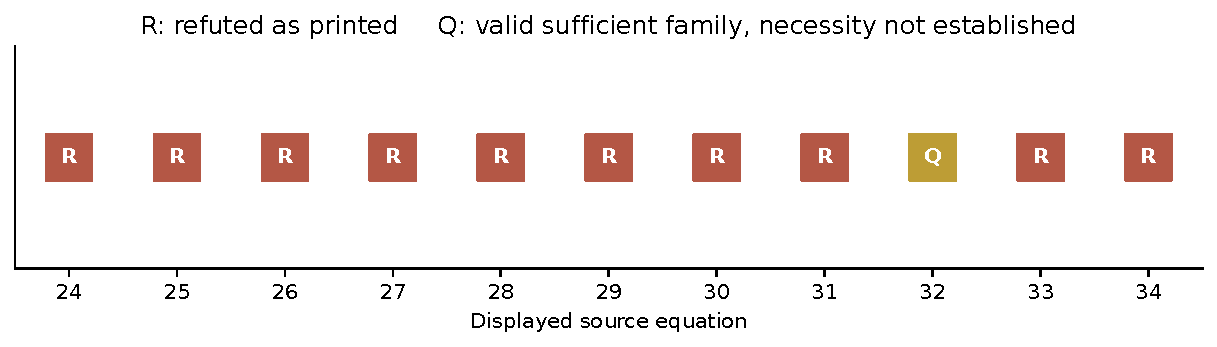
\includegraphics[width=.96\textwidth]{source-audit.pdf}
\caption{Source audit on declared charts. Refutations have retained exact witnesses. The qualified formula supplies a sufficient family.}\label{fig:audit}\end{figure}
The cubic quotient also requires a corrected chain rule and a separate singular branch (Appendix~\ref{app:algebra}). An integration constant must be retained: fixing it silently replaces a general family by one member.

The Eulerian source \cite{sve2022}, equation (25), prints $t\partial_t-2u\partial_u-h\partial_h-2B\partial_B$ for cubic transport. Its bed-equation tangency residual is $-9\kappa u^2u_x$, which is not identically zero. The corrected comparison $t\partial_t-u\partial_u-2h\partial_h-2B\partial_B$ has zero residual in all three original equations. Separately, mixing a general-exponent substitution rule with a cubic equation produced the historical implementation witness $-6$. The source-formula discrepancy and that implementation defect are different failures; neither establishes full reproduction of every Eulerian reduction.

\section{Strict discovery: what is established}
The strict input is the PDE with arbitrary point coefficients, without a supplied generator basis or polynomial degree bound. Two prolongation formulas agree. Returned finite families are independently substituted into the determining equations and original-PDE tangency conditions. Inputs cover eight one-dimensional cells, seventeen two-dimensional cells, three scalar inputs and two mixed-law inputs.

In the initial campaign, twenty-nine inputs returned families; the generic one-dimensional Grass input timed out at 60, 300 and 1800 seconds. Across those outputs, 44 finite families pass residual and bracket checks and four $m=0$ branches are excluded by their declared $1\le m\le4$ domains. These are branch counts, not 44 independent PDE models. Terminal conditions are matched to returned families independently of output order. Fixed-parameter and first-jet guards are parsed. This correspondence does not prove that every parameter branch has been found.
\begin{figure}[htbp]\centering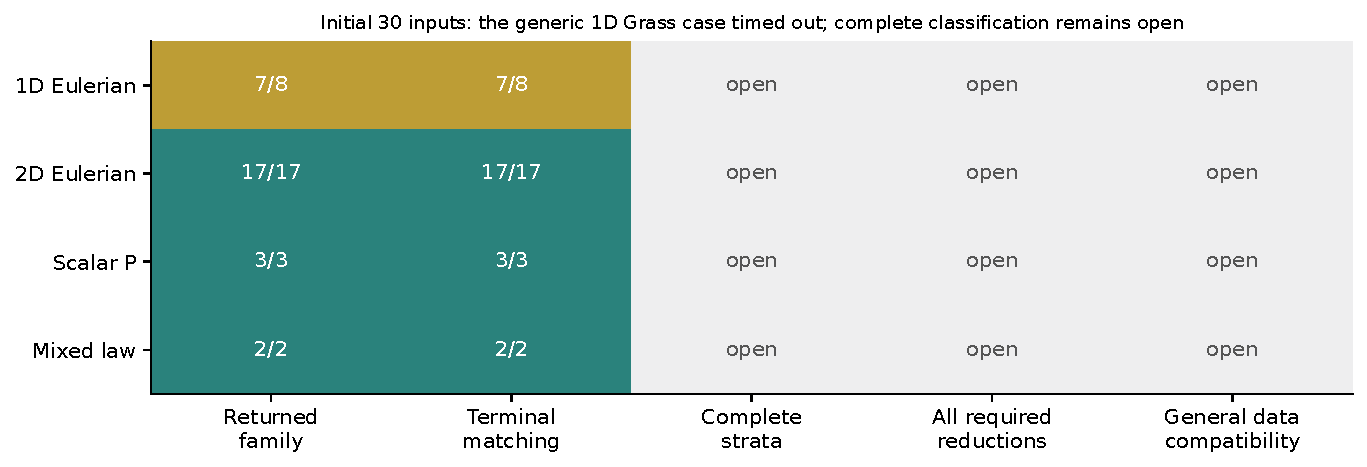
\includegraphics[width=\textwidth]{strict-coverage.pdf}
\caption{Capability gates. Checked families are admitted on stated conditions. Complete parameter classification and general data compatibility remain open.}\label{fig:coverage}\end{figure}
For the nine source-selected subgroups at general $m$, $m=1$ and $m=3$, every defined final characteristic/pullback identity vanishes. Selectors are compared with the computed algebra only after solving. Undefined charts, no-graph cases and absent generators remain explicit. A stationary identity at $m=1$ or $3$ does not satisfy the positive-velocity chart. Selected certificates do not constitute an exhaustive reduction classification.

The translation reducer records 38 implicit ODE/DAE chains, five actions with no invariant graph in the declared chart, and one undefined chart. Defined reconstruction identities vanish after preserving parameter guards and using positive-base power identities. These counts concern selected branches; an implicit system is not automatically a regular ODE with a solved initial-value problem.

A native retry supplied the same thirty independently derived determining equations directly to CRACK. With physical coefficients fixed symbolically, it returned in 3.90 seconds. Independent substitution and brackets verify a four-dimensional algebra, with span
\begin{equation}\langle\partial_t,\partial_x,\partial_B,t\partial_t+x\partial_x\rangle.\end{equation}
The returned parameterization has poles at $m=1,2$; together with the input conditions, this certificate uses $1\le m\le4$, $m\notin\{1,2,3\}$. Separate solves at $m=1$ retain a differential equation, while $m=2$ returns unevaluated integrals and function dependencies that the current verifier cannot certify. The generic chart also gives one additional exact translation reduction, but these results do not close the whole Grass cell.
\begin{figure}[htbp]\centering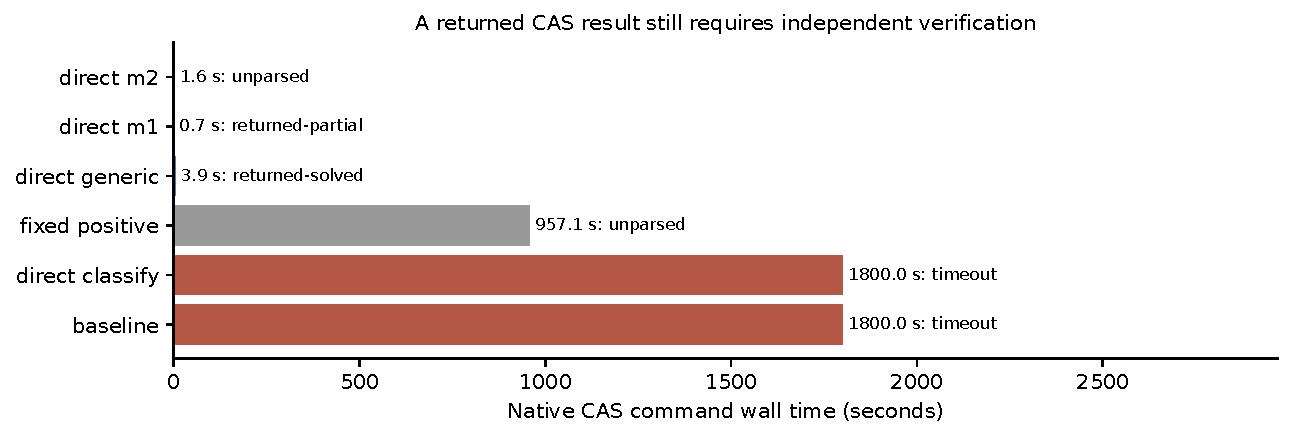
\includegraphics[width=.94\textwidth]{remote-runtime.pdf}
\caption{Recorded CAS times. The original and classification runs timed out. Another run exited without a final result, while the generic direct solve required a parser repair before independent verification. Exceptional-layer returns remain incomplete. Formulations and memory limits differ, so these bars do not measure hardware speedup.}\label{fig:runtime}\end{figure}
The cumulative CAS time was 4564.4 seconds under a 7200-second cap. One timeout's process-cleanup check failed and the original controller continued; later absence of processes cannot certify that transition. The repaired controller stops on unconfirmed cleanup. A zero exit code without a complete result is never accepted as a mathematical solution.

\section{Failures and academic acceptance}
\begin{table}[htbp]\centering\small
\begin{tabularx}{\textwidth}{@{}lX@{}}\toprule
Outcome & Meaning\\\midrule
Nonzero tangency/pullback & The candidate or formula fails on the stated model.\\
Zero denominator/rank loss & The chosen chart is invalid; retain the undivided equation.\\
No invariant graph & This action has no graph on that chart; other actions remain possible.\\
Implicit ODE/DAE & Reduction exists; regular solvability needs a leading-matrix check.\\
Timeout/incomplete output & Computationally unresolved, not a nonexistence proof.\\
Unchecked data stabilizer & Invariance of the same initial-boundary problem is unproved.\\\bottomrule
\end{tabularx}\caption{Different failures require different conclusions.}
\end{table}
A selected reduction needs explicit hypotheses, characteristic integration and independent reconstruction. The complete declared classification additionally needs a necessary-and-sufficient determining-system solution and coverage of exceptional strata. Numerical pointwise agreement is a diagnostic, not a continuous PDE-error theorem. Reduced ODEs need not have elementary closed-form general solutions.

\section{Elimination methods that preserve the problem}
Wolf's length-reduction method combines equations to remove large common expressions before differential elimination \cite{wolf2002}. Each replacement must preserve the solution set; every divided factor must be nonzero or split into another branch. Thomas decomposition handles equations and inequations together and checks differential compatibility within each simple subsystem \cite{thomas2010}. Its published implementation uses Maple; this work uses REDUCE and does not claim to have run Maple.

LIEPDE distinguishes fixed symbolic coefficients from parameters to be classified \cite{liepde}. Treating all parameters as unknowns can create difficult nonlinear branches. The alternatives retain arbitrary generator functions while feeding independently split determining equations to CRACK, or treating known-positive coefficients as symbolic coefficients. Generic solutions still require exceptional-parameter analysis. No generator degree is prescribed.

On $u>0$, distinct powers $u^{a_j(m)}$ can be separated only after the determining equations establish the relevant coefficient dependencies. Exponent collisions generate strata; parameter sampling cannot prove their absence. Characteristic equations then yield similarity variables, whose independence and coordinate rank must be checked.

\section{Classical computation before learning}
A regular first-integral chart supplies a classical ODE baseline. Learning must include the same derivative, residual and data checks. With setup costs $T_N,T_C$ and full query costs $q_N,q_C$, it wins only if $(T_N-T_C)+n(q_N-q_C)<0$. Pure PINN is stopped; inherited unmatched counts establish no performance advantage. New learning requires an unmet task and a frozen matched-accuracy comparison.
\chapter{Extensions}\label{ch:outlook}
\section{A constructed annular Eulerian reference}\label{sec:2d}
Consider smooth two-dimensional flow with constant Coriolis parameter $f$ and cubic transport with downslope diffusion,
\begin{align}
h_t+\nabla\!\cdot(h\mathbf w)&=0,\\
\mathbf w_t+(\mathbf w\!\cdot\nabla)\mathbf w+g\nabla(h+B)+f\mathcal J\mathbf w&=0,\\
B_t+\nabla\!\cdot\{K|\mathbf w|^2\mathbf w-G|\mathbf w|^2\nabla B\}&=0,
\end{align}
where $\mathcal J(u,v)=(-v,u)$ and $g,K,G>0$. Joint rotation
$J=-y\partial_x+x\partial_y-v\partial_u+u\partial_v$ and $T+c\partial_B$ have projection rank two on $r=\sqrt{x^2+y^2}>0$. Invariant graphs take the form
\begin{equation}h=H(r),\quad\mathbf w=V(r)\mathbf e_r+W(r)\mathbf e_\theta,\quad B=Z(r)+ct.\end{equation}
This supplied-subalgebra benchmark was checked independently before the strict discovery campaign; it does not certify automatic maximal classification. Substitution gives
\begin{align}
(rHV)'&=0,\\
VV'-W^2/r-fW+g(H'+Z')&=0,\\
V(W'+W/r+f)&=0,\\
c+(rq_r)'/r&=0,\qquad q_r=(V^2+W^2)(KV-GZ').
\end{align}
On $H,V>0$, $V^2-gH\ne0$ and $G(V^2+W^2)\ne0$, a regular five-state ODE results. Three independent first integrals are
\begin{equation}rHV=C_1,\qquad rW+fr^2/2=C_2,\qquad rq_r+cr^2/2=C_3.\end{equation}
Independent Cartesian differentiation verifies reconstruction. The normal used for $q_r$ points away from the origin; the domain-outward normal at an inner annular boundary has opposite sign.

For $(g,K,G,f,c)=(1,.05,.1,.2,.02)$ and initial data $(H,V,W,Z,Z')=(1,2,.3,0,.9)$ at $r=1$, the recorded integration covers $1\le r\le1.25$ with DOP853 \cite{hairer} tolerances $10^{-12}$ and $10^{-14}$. The minimum depth is approximately $0.801$ and the minimum absolute characteristic pivot is $3$.
\begin{figure}[htbp]\centering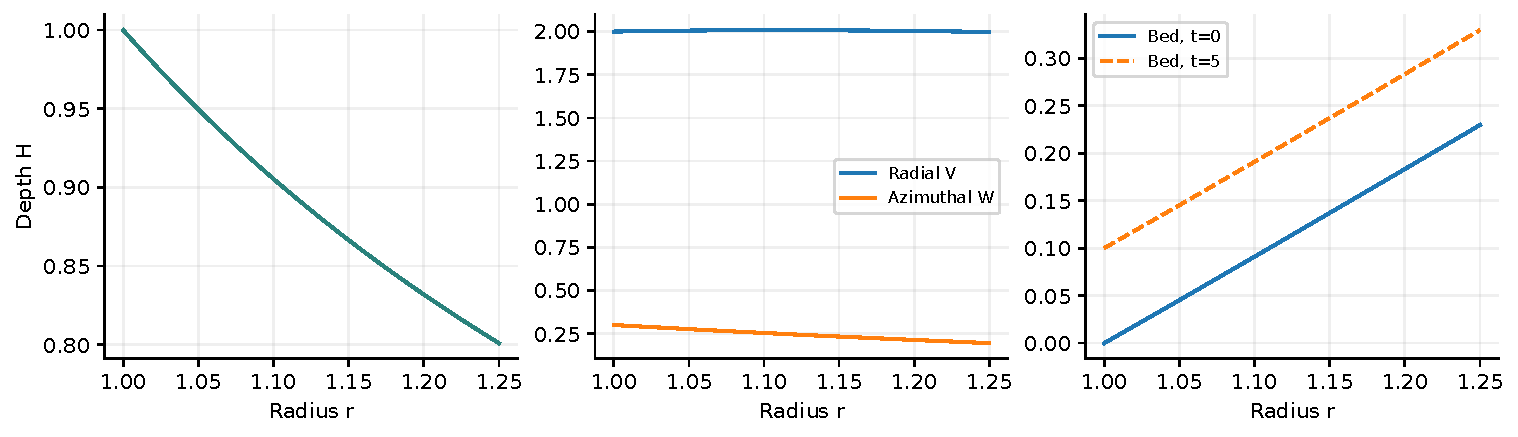
\includegraphics[width=\textwidth]{annular-fields.pdf}
\caption{Constructed annular fields, not observations. Bed evolution is $B=Z+.02t$.}\label{fig:annular}\end{figure}
\begin{figure}[htbp]\centering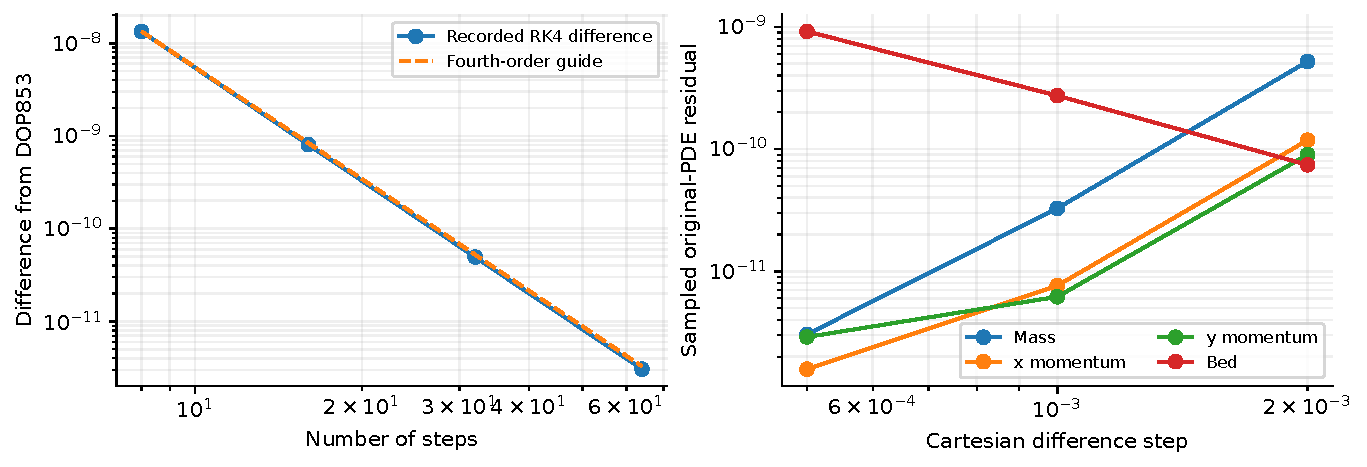
\includegraphics[width=\textwidth]{annular-verification.pdf}
\caption{RK4 refinement against DOP853 and sampled Cartesian residuals. The bed residual worsens at the smallest difference step. Neither panel certifies continuous PDE error.}\label{fig:annular-checks}\end{figure}
The finest displayed RK4 difference is approximately $3.06\times10^{-12}$; first-integral drifts are below $10^{-14}$. Constructed circular boundary data are compatible with the chosen actions. Arbitrary initial-boundary data are not covered.

\section{Independent mixed-law transfer}
Retain the water equations and replace the sediment flux by
\begin{equation}\mathbf q=(K_1+K_3|\mathbf w|^2)\mathbf w-G|\mathbf w|^2\nabla B,\qquad K_1,K_3,G>0.\end{equation}
Separate arbitrary-coefficient inputs at fixed $f=0$ and $f\ne0$ return a five-dimensional admitted family containing time, spatial and bed translations and joint rotation. Independent prolongation accepts joint rotation and rejects spatial-only rotation. The old cubic dilation
\begin{equation}S=x\partial_x+y\partial_y+u\partial_u+v\partial_v+2h\partial_h+2B\partial_B\end{equation}
has bed tangency defect
\begin{equation}\boxed{-2K_1(u_x+v_y).}\end{equation}
It fails generically. The linear transport term breaks scaling while rotational covariance remains. Selected translation pullbacks are available; complete characteristic-to-reconstruction coverage is open. The earlier annular profile is not reused as a solved profile of this new law.
\section{An inverse symmetry problem for the Eulerian system}
The previous chapters hold $q=\kappa u^m$ fixed and solve for transformations or profiles. A different problem leaves $q(h,u)$ unknown while preserving \eqref{eq:e1}--\eqref{eq:e3}. Consider the candidate generator
\begin{equation}\label{eq:euler-scale}
S=x\partial_x+u\partial_u+2h\partial_h+2B\partial_B.
\end{equation}
Its flow fixes time and maps $(x,u,h,B)$ to $(\lambda x,\lambda u,\lambda^2h,\lambda^2B)$, $\lambda>0$, with $g$ fixed. Continuity scales by $\lambda^2$ and primitive momentum by $\lambda$. Exner requires the flux derivative to scale by $\lambda^2$.

\begin{proposition}[Scale-compatible local fluxes]\label{prop:closure}
Let $q\in C^2$ on a connected scaling-invariant local region with $h>0$. The Eulerian system admits \eqref{eq:euler-scale} if and only if
\begin{equation}\label{eq:closure-condition}
2h q_h+u q_u-3q=C
\end{equation}
for a state-independent constant $C$. Up to an additive constant flux, its general local solution is
\begin{equation}\label{eq:closure-family}
q(h,u)=\sqrt g\,h^{3/2} f\!\left(\frac{u}{\sqrt{gh}}\right),
\end{equation}
where $f$ is an arbitrary sufficiently smooth function on the corresponding invariant interval.
\end{proposition}
\begin{proof}
Let $D=2h\partial_h+u\partial_u$. For $q_x=q_hh_x+q_uu_x$, prolonged scaling gives $\pr S(q_x)=D_x(Dq)-q_x$, while $\pr S(B_t)=2B_t$. Thus
\begin{equation}
\pr S(B_t+q_x)-2(B_t+q_x)=D_x(Dq-3q).
\end{equation}
The time derivatives are solved by the three first-order field equations, leaving $h_x,u_x$ free. Hence the last expression vanishes identically on the equation locus if and only if $(Dq-3q)_h=(Dq-3q)_u=0$, proving \eqref{eq:closure-condition}. Replacing $q$ by $\widetilde q=q+C/3$ leaves $q_x$ unchanged and gives $D\widetilde q=3\widetilde q$.

Along characteristics $\dot h=2h$, $\dot u=u$, $\dot{\widetilde q}=3\widetilde q$, the ratios $r=u/\sqrt{gh}$ and $\widetilde q/(\sqrt g\,h^{3/2})$ are constant. Thus the second ratio is an arbitrary function of the first, proving \eqref{eq:closure-family}. Direct differentiation proves sufficiency.\end{proof}
Here $r$ is a signed Froude variable; on the positive-velocity benchmark it is positive. The prefactor has flux units $L^2/T$. Dimensionless material parameters may be additional arguments of $f$. If a reference state supplies an absolute sediment flux, the otherwise invisible additive constant is fixed by that datum.

If $q$ depends on $u$ alone, differentiating \eqref{eq:closure-condition} gives $uq_{uu}-2q_u=0$, hence $q=\kappa u^3+q_0$ on a connected nonzero-velocity interval. For a power law, the derivative constraint is $\kappa m(m-3)u^{m-1}=0$. The $m=0$ solution is a constant flux with zero interior divergence; excluding it is a nondegenerate transport assumption, not an algebraic omission.

\chapter{Conclusions and Future Work}
\section{Answers to the research questions}
The printed and corrected scalar equations are different models. Only a reconstruction certificate supports a claim about the full Eulerian system. The common-scaling example shows how characteristic integration removes one independent variable and how a separate first integral lowers ODE order.

Source reproduction produced corrections and exact negative witnesses. The strict backend checks returned families and selected reductions, but the full classification remains incomplete. A timeout does not establish absence of symmetry. The annular example has an exact reduction and sampled numerical verification on a regular chart, not general two-dimensional solvability or physical validation. For the independently posed mixed law, rotation survives and the old cubic scaling fails.

The resulting workflow is symmetry first: define the model and chart, derive or verify the action, reduce, reconstruct, and then compare approximation costs. No neural superiority or universal reduction success is claimed.
\section{Next falsifiable tasks}
First complete the generic Grass determining system and exceptional-parameter coverage. Then extend characteristic integration beyond selected actions and certify projection ranks and singular branches. Check the stabilizer of an unchanged initial-boundary problem separately from invariant-solution trace compatibility. Only when verified classical reduction leaves a measurable unmet task should a learned object be compared with a classical control. A documented failure at any of these gates remains an informative result.
\appendix
\chapter{Technical Derivations}\label{app:algebra}
\section{The cubic chart and a corrected chain rule}\label{sec:cubic}
For model $P$ at $m=3$, the flow of $X_5$ is
$(t,s,\phi)\mapsto(e^\varepsilon t,e^{-2\varepsilon}s,\phi)$.
On $t>0$, $z=st^2$ and $\phi$ are invariants. The characteristic is
$Q=-t\phi_t+2s\phi_s$, so $Q=0$ gives $\phi=F(z)$.
Direct substitution yields
\begin{equation}\label{eq:cubic}
\E_3^{\mathrm p}=t^{-1}\R_5,\qquad
\R_5=2zA_5'-g\beta B_5',\quad\beta=3\kappa,
\end{equation}
where
\begin{equation}
A_5=2zp^2+4z^2pc-gc/p^2,\qquad
B_5=8z^2p(p+zc).
\end{equation}
To use fractional-power differential invariants restrict to $z>0$ and define
\begin{equation}
\Sigma=z^{2/3}p,\qquad \mathsf M=z^{5/3}c,
\qquad W=\mathsf M+\tfrac23\Sigma.
\end{equation}
Their derivatives are
\begin{equation}
\Sigma'=z^{-1}W,\qquad
\mathsf M'=z^{5/3}H+\tfrac53z^{2/3}c,
\quad H=F'''(z).
\end{equation}
Therefore the correct quotient formula is
\begin{equation}\boxed{\displaystyle
\frac{\dd\mathsf M}{\dd\Sigma}
=\frac{z^{8/3}H+\tfrac53\mathsf M}{W}.}\label{eq:chain-correct}
\end{equation}
The factor $W$ determines whether $\Sigma$ is a valid local independent variable. The power $z^{8/3}$ in \eqref{eq:chain-correct} follows from differentiating the definitions, independently of any normal-form division.

If $W\equiv0$ on an interval, $zp'+\tfrac23p=0$ gives
$F=C+Kz^{1/3}$. Substitution into \eqref{eq:cubic} on the positive branch fixes
\begin{equation}\label{eq:power}
K^3=\frac{27g}{1-4g\beta}=\frac{27g}{1-12g\kappa},\qquad 1-12g\kappa>0.
\end{equation}
Thus the amplitude is constrained. At $g=1$, $\kappa=1/30$, $K^3=45$. An isolated zero of $W$ is instead a chart turning point and need not define this entire power-law branch. On $W\ne0$, the quotient relation can be expressed as an Abel equation in $N=1/W$; Appendix~\ref{app:algebra} gives its explicit coefficients.

\section{The regular cubic quotient and Abel coefficients}
Write $a=g\beta$, $s_*=\Sigma$ temporarily, and
$D(s_*)=4(1-a)s_*^3-g$. Substituting the normal-form expression for $H$ from \eqref{eq:cubic} into \eqref{eq:chain-correct} gives
\begin{equation}\label{eq:quotient-explicit}
\frac{\dd\mathsf M}{\dd s_*}=
\frac{12(a-1)\mathsf M^2s_*^3-6g\mathsf M^2
 +(40a-16)\mathsf M s_*^4-5g\mathsf M s_*
 +(24a-6)s_*^5}{s_*(3\mathsf M+2s_*)D(s_*)}.
\end{equation}
The regular positive chart requires $s_*>0$, $W\ne0$, $D\ne0$. Setting $N=1/(\mathsf M+2s_*/3)$ and differentiating gives
\begin{equation}
N'=f_1N+f_2N^2+f_3N^3,
\end{equation}
where
\begin{align}
f_1(s_*)&=\frac{4(1-a)s_*^3+2g}{s_*D(s_*)},\\
f_2(s_*)&=-\frac{(16a+8)s_*^3+g}{3D(s_*)},\\
f_3(s_*)&=-\frac{2s_*[(4a-1)s_*^3+g]}{9D(s_*)}.
\end{align}
These are local formulas; no generic closed-form solution of the Abel equation is claimed. Once $\mathsf M(s_*)$ is known, reconstruct $z$ from
$\dd\log z/\dd s_*=1/W=N$, then recover $F'$ from $s_*=z^{2/3}F'$. The $W\equiv0$ branch is excluded by this coordinate change and is retained separately in \eqref{eq:power}. Points with $D=0$ also require the undivided residual.

\section{First-integral defects and reconstructed errors}
For a candidate $\widehat F$ define $r_I=L_m(z,\widehat F,\widehat F')\widehat F''-I_0$. The original reduced residual is exactly $r_I'$. Consequently, small $\norm{r_I}_{L^2}$ alone does not control $\norm{r_I'}_{L^2}$. For example $r_I=\varepsilon\sin(kz)$ has small amplitude but derivative amplitude $\varepsilon k$. A first-integral training objective therefore still requires independent third-order residual verification if that is the declared acceptance criterion.

Similarly, $h=1/p$ implies
$|\widehat h-h|\le|\widehat p-p|/p_{\min}^2$ only when both slopes remain above a uniform positive $p_{\min}$. This guard has physical meaning: it protects the invertibility and conditioning of the mass-coordinate map.

\clearpage
\addcontentsline{toc}{chapter}{Bibliography}
\begingroup\small\singlespacing
\setlength{\bibsep}{3pt plus 1pt minus 1pt}
\begin{thebibliography}{99}
\providecommand{\natexlab}[1]{#1}
\newcommand{\doi}[1]{\url{https://doi.org/#1}}

\bibitem[Olver(1993)]{olver}
Peter~J. Olver.
\newblock \emph{{Applications of Lie Groups to Differential Equations}}.
\newblock Springer, 2 edition, 1993.
\newblock \doi{10.1007/978-1-4612-4350-2}.

\bibitem[Olver(1986)]{olver1986}
Peter~J. Olver.
\newblock \emph{Applications of Lie Groups to Differential Equations}.
\newblock Springer, first edition, Graduate Texts in Mathematics 107, 1986.
\newblock \doi{10.1007/978-1-4684-0274-2}.


\bibitem[Oliveri(2026)]{oliveri2026}
Francesco Oliveri.
\newblock \emph{{Lie Symmetries of Differential Equations: Theory,
  Applications, and Symbolic Computation}}.
\newblock Birkh{\"a}user, 2026.
\newblock \doi{10.1007/978-3-032-12791-4}.

\bibitem[Anderson et~al.(2000)Anderson, Fels, and Torre]{anderson2000}
Ian~M. Anderson, Mark~E. Fels, and Charles~G. Torre.
\newblock {Group Invariant Solutions without Transversality}.
\newblock \emph{Communications in Mathematical Physics}, 212\penalty0
  (3):\penalty0 653--686, 2000.
\newblock \doi{10.1007/s002200000215}.
\newblock URL \url{https://arxiv.org/abs/math-ph/9910015}.

\bibitem[Paliathanasis et~al.(2026)Paliathanasis, Leon, and Leach]{ap}
Andronikos Paliathanasis, Genly Leon, and Peter G.~L. Leach.
\newblock {Lie Symmetries and Similarity Solutions for a Shallow-Water Model
  with Bed Elevation in Lagrange Variables}.
\newblock \emph{Mathematics}, 14:\penalty0 433, 2026.
\newblock \doi{10.3390/math14030433}.

\bibitem[Teschl(2012)]{teschl2012}
Gerald Teschl.
\newblock \emph{Ordinary Differential Equations and Dynamical Systems}, volume
  140 of \emph{Graduate Studies in Mathematics}.
\newblock American Mathematical Society, Providence, 2012.
\newblock ISBN 978-0-8218-8328-0.
\newblock URL \url{https://www.mat.univie.ac.at/~gerald/ftp/book-ode/}.

\bibitem[Paliathanasis(2022)]{sve2022}
Andronikos Paliathanasis.
\newblock Lie Symmetry Analysis of the One-Dimensional Saint-Venant-Exner Model.
\newblock \emph{Symmetry}, 14:1679, 2022.
\newblock \doi{10.3390/sym14081679}.

\bibitem[Lagaris et~al.(1998)Lagaris, Likas, and Fotiadis]{lagaris}
I.~E. Lagaris, A.~Likas, and D.~I. Fotiadis.
\newblock {Artificial Neural Networks for Solving Ordinary and Partial
  Differential Equations}.
\newblock \emph{IEEE Transactions on Neural Networks}, 9:\penalty0 987--1000,
  1998.
\newblock URL \url{https://arxiv.org/abs/physics/9705023}.

\bibitem[Mishra and Molinaro(2023)]{mishra2023}
Siddhartha Mishra and Roberto Molinaro.
\newblock Estimates on the generalization error of physics-informed neural
  networks for approximating pdes.
\newblock \emph{IMA Journal of Numerical Analysis}, 43\penalty0 (1):\penalty0
  1--43, 2023.
\newblock \doi{10.1093/imanum/drab093}.
\newblock URL \url{https://arxiv.org/abs/2006.16144}.

\bibitem[Akhound-Sadegh et~al.(2023)Akhound-Sadegh, Perreault-Levasseur,
  Brandstetter, Welling, and Ravanbakhsh]{sympinn}
Tara Akhound-Sadegh, Laurence Perreault-Levasseur, Johannes Brandstetter, Max
  Welling, and Siamak Ravanbakhsh.
\newblock {Lie Point Symmetry and Physics Informed Networks}.
\newblock In \emph{Advances in Neural Information Processing Systems},
  volume~36, 2023.
\newblock URL \url{https://arxiv.org/abs/2311.04293}.

\bibitem[Otto et~al.(2025)]{otto}
Samuel E. Otto, Nicholas Zolman, J. Nathan Kutz, and Steven L. Brunton.
\newblock A Unified Framework to Enforce, Discover, and Promote Symmetry in Machine Learning.
\newblock \emph{Journal of Machine Learning Research}, 26(248):1--83, 2025.
\newblock \url{https://jmlr.org/papers/v26/24-1315.html}.

\bibitem[Hairer(software)]{hairer}
Ernst Hairer.
\newblock Fortran and Matlab Codes: DOP853, explicit Runge--Kutta method of order 8(5,3).
\newblock Author-maintained software documentation, University of Geneva.
\newblock \url{https://www.unige.ch/~hairer/software.html}.

\bibitem[Trefethen(2000)]{trefethen}
Lloyd N. Trefethen.
\newblock \emph{Spectral Methods in MATLAB}.
\newblock SIAM, Philadelphia, 2000.
\newblock \doi{10.1137/1.9780898719598}.

\bibitem[Wolf(2002)]{wolf2002} Thomas Wolf. Size reduction and partial decoupling of systems of equations. \emph{Journal of Symbolic Computation}, 33(3):367--383, 2002. \href{https://arxiv.org/abs/cs/0301029}{arXiv:cs/0301029}.
\bibitem[B\"achler et al.(2010)]{thomas2010} Thomas B\"achler, Vladimir Gerdt, Markus Lange-Hegermann and Daniel Robertz. Thomas decomposition of algebraic and differential systems, 2010. \href{https://arxiv.org/abs/1008.3767}{arXiv:1008.3767}.
\bibitem[Wolf(1993)]{liepde} Thomas Wolf. An efficiency improved program LIEPDE for determining Lie symmetries of PDEs. In \emph{Modern Group Analysis}, pp.\ 377--385, Kluwer, 1993.

\end{thebibliography}
\endgroup
\end{document}
